%!TEX root = ./main.tex
%
% This file is part of the i10 thesis template developed and used by the
% Media Computing Group at RWTH Aachen University.
% The current version of this template can be obtained at
% <http://www.media.informatik.rwth-aachen.de/karrer.html>.

\chapter{Hardware Prototype and Software }
\label{ownwork} 


In this chapter we present the construction of the hardware setup and the user study software. 
Furthermore we talk about the technical considerations regarding each component and their feasibility.


\section{System Design}
The aim of this thesis is to investigate the perception of several feedback modalities underwater and their feasibility for low level navigation cues.
We include visual, auditory, and tactile feedback in form of a LED, waterproof in ear headphones,  a vibration motor, and a thermoelectric cooling module.
The prototype has to incorporate these methods as unobtrusive and comfortable as possible in particular when they are  inactive. 
Electronic connections have to be waterproof, undisturbing, and fail safe.
Furthermore all components should be affordable to provide an advantage over commercial solutions.

To investigate the recognition times and comfort of each technique we built a prototype composed of one LED in the diving goggles as well as a waterproof vibration motor and a Peltier cooling module in a stretchable headband.
The headphones are provided separately.

\paragraph{Visual Feedback}

To provide visual low level feedback we use a common red 5 mm LED.
An issue regarding luminous light emitted by an LED is its proneness to water reflections.
These reflections change rapidly due to water undulation and exterior lighting.
The color of the surroundings influence it as well.
For example light blue tiles in a swimming pool render a blue LED almost undetectable.
To provide clear recognizable feedback we tested several colors underwater and came to the conclusion that red LED is better recognizable than other common LED colors.

There are several ways to provide feedback with an LED.
Depending on the way it is presented the user might not notice it fast enough if the brightness increases over time.
However, this might be more comfortable than turning on the LED to full brightness instantly.
Therefore we implement both.
First we set the bright from to full brightness immediately.
Second we increase the brightness from 0\% to 100\%  and back to 0\% over 5.1 seconds resulting in a slowly blinking pattern.
We choose this interval arbitrarily after testing several duration.
This can be further investigated but would go beyond the scope of this thesis since we aim to consider several modalities.


\paragraph{Auditory Feedback}

For auditory feedback we choose AGPTEK E11B IPX8 waterproof in-ear headphones.
The headphones are worn separately from the other components and are connected to the operating MacBook Pro.
Like visual feedback, the comfortability of auditory feedback depends on the way it is presented to the user. 
The audio file played should start immediately and be clearly recognizable.
Furthermore the pitch and loudness should be within an appropriate range.
We use the sound of a sonar since it suits the underwater scenario.


\paragraph{Vibration Feedback}

To provide feedback using vibration actuators we choose waterproof 7 mm vibration motors.
They are working at 3.3V with 2.45g at 250Hz.
We tried to make smaller vibration motors waterproof.
Using shrinking tubing and epoxy resin adhesive made them waterproof but running them over night underwater let them stop working regardless.
Thus we have to stick to the larger motor.

We handle the vibration feedback similar to the visual feedback and set it to maximum power instantaneously as well as increasing it over time.
Test have shown that it requires a certain amount of voltage to feel a vibration even outside the water.
Therefore we start at 1,18V and increase to 3.3V over 5.4 seconds.


\paragraph{Thermal Feedback}

For thermal feedback we choose a CUI CP6014 Thermoelectric Module. 
\cite{Peiris_thermoVR} have shown that users prefer cooling over heating.
Cooling also performs better when it comes to recognition time.
Previously we tested heating and cooling effects in water with 21 degrees and cooling was much faster perceivable than heating.
Additionally heating effects were rarely recognizable.
The Peltier module has a maximum voltage of 2.1V and maximum current of 6A.
Therefore we use an external battery combined with a relay to run it.
There are specific circuit boards to control the temperature of thermoelectric cooing elements.
However we considered that running it on full power is sufficient for our purpose since we are interested in the fastest possible reaction times underwater.


\subsection{Hardware Prototype}
\todo{more pictures of prototype creation and the electronics}

As shown in figure~\ref{fig:ledcloseup} the LED is glued to the diving goggles between the silicone and the frame.
There are three reasons to place the LED there.
First, the LED is not in sight or noticeable when turned off and thus unobtrusive.
Second, the light is diffused by the silicone leading to non-dazzling feedback.
Third, the cable routing is easier compared to placing it within the silicone and still make sure no water gets in.

\begin{figure}
	\includegraphics[width= \textwidth]{images/LEDcloseupcut.png}
	\caption{LED insulated and attached between the silicone and frame of the diving goggles using hotglue. }~\label{fig:ledcloseup}
\end{figure}

In addition to the stretchability of the headband it features \todo{length of fastener} a pair of hook and loop fastener as shown in figure~\ref{fig:headbandfastener}.
This enables adjustable, tight, and still comfortable wear of the headband.
The fasteners were sewn to the 40mm wide elastic band using a Bernina 880.

\begin{figure}
	\includegraphics[width= \textwidth]{images/headbandfastener.png}
	\caption{Stretchable headband with hook and loop fastener+ sewn to it. Allows comfortable adjustment on different head froms and sizes.}~\label{fig:headbandfastener}
\end{figure}

To sense the cooling effect of the thermoelectric module it has to be placed directly onto the users skin.
We achieve this by cutting two holes in the elastic band and put the VCC and Ground wires through it. 
Although the edges of the module seem to be uncomfortable, none of the users noticed it at all while it was turned off.
The heat produced by the Peltier element is no issue underwater since the water naturally conducts the heat away.

\begin{figure}
	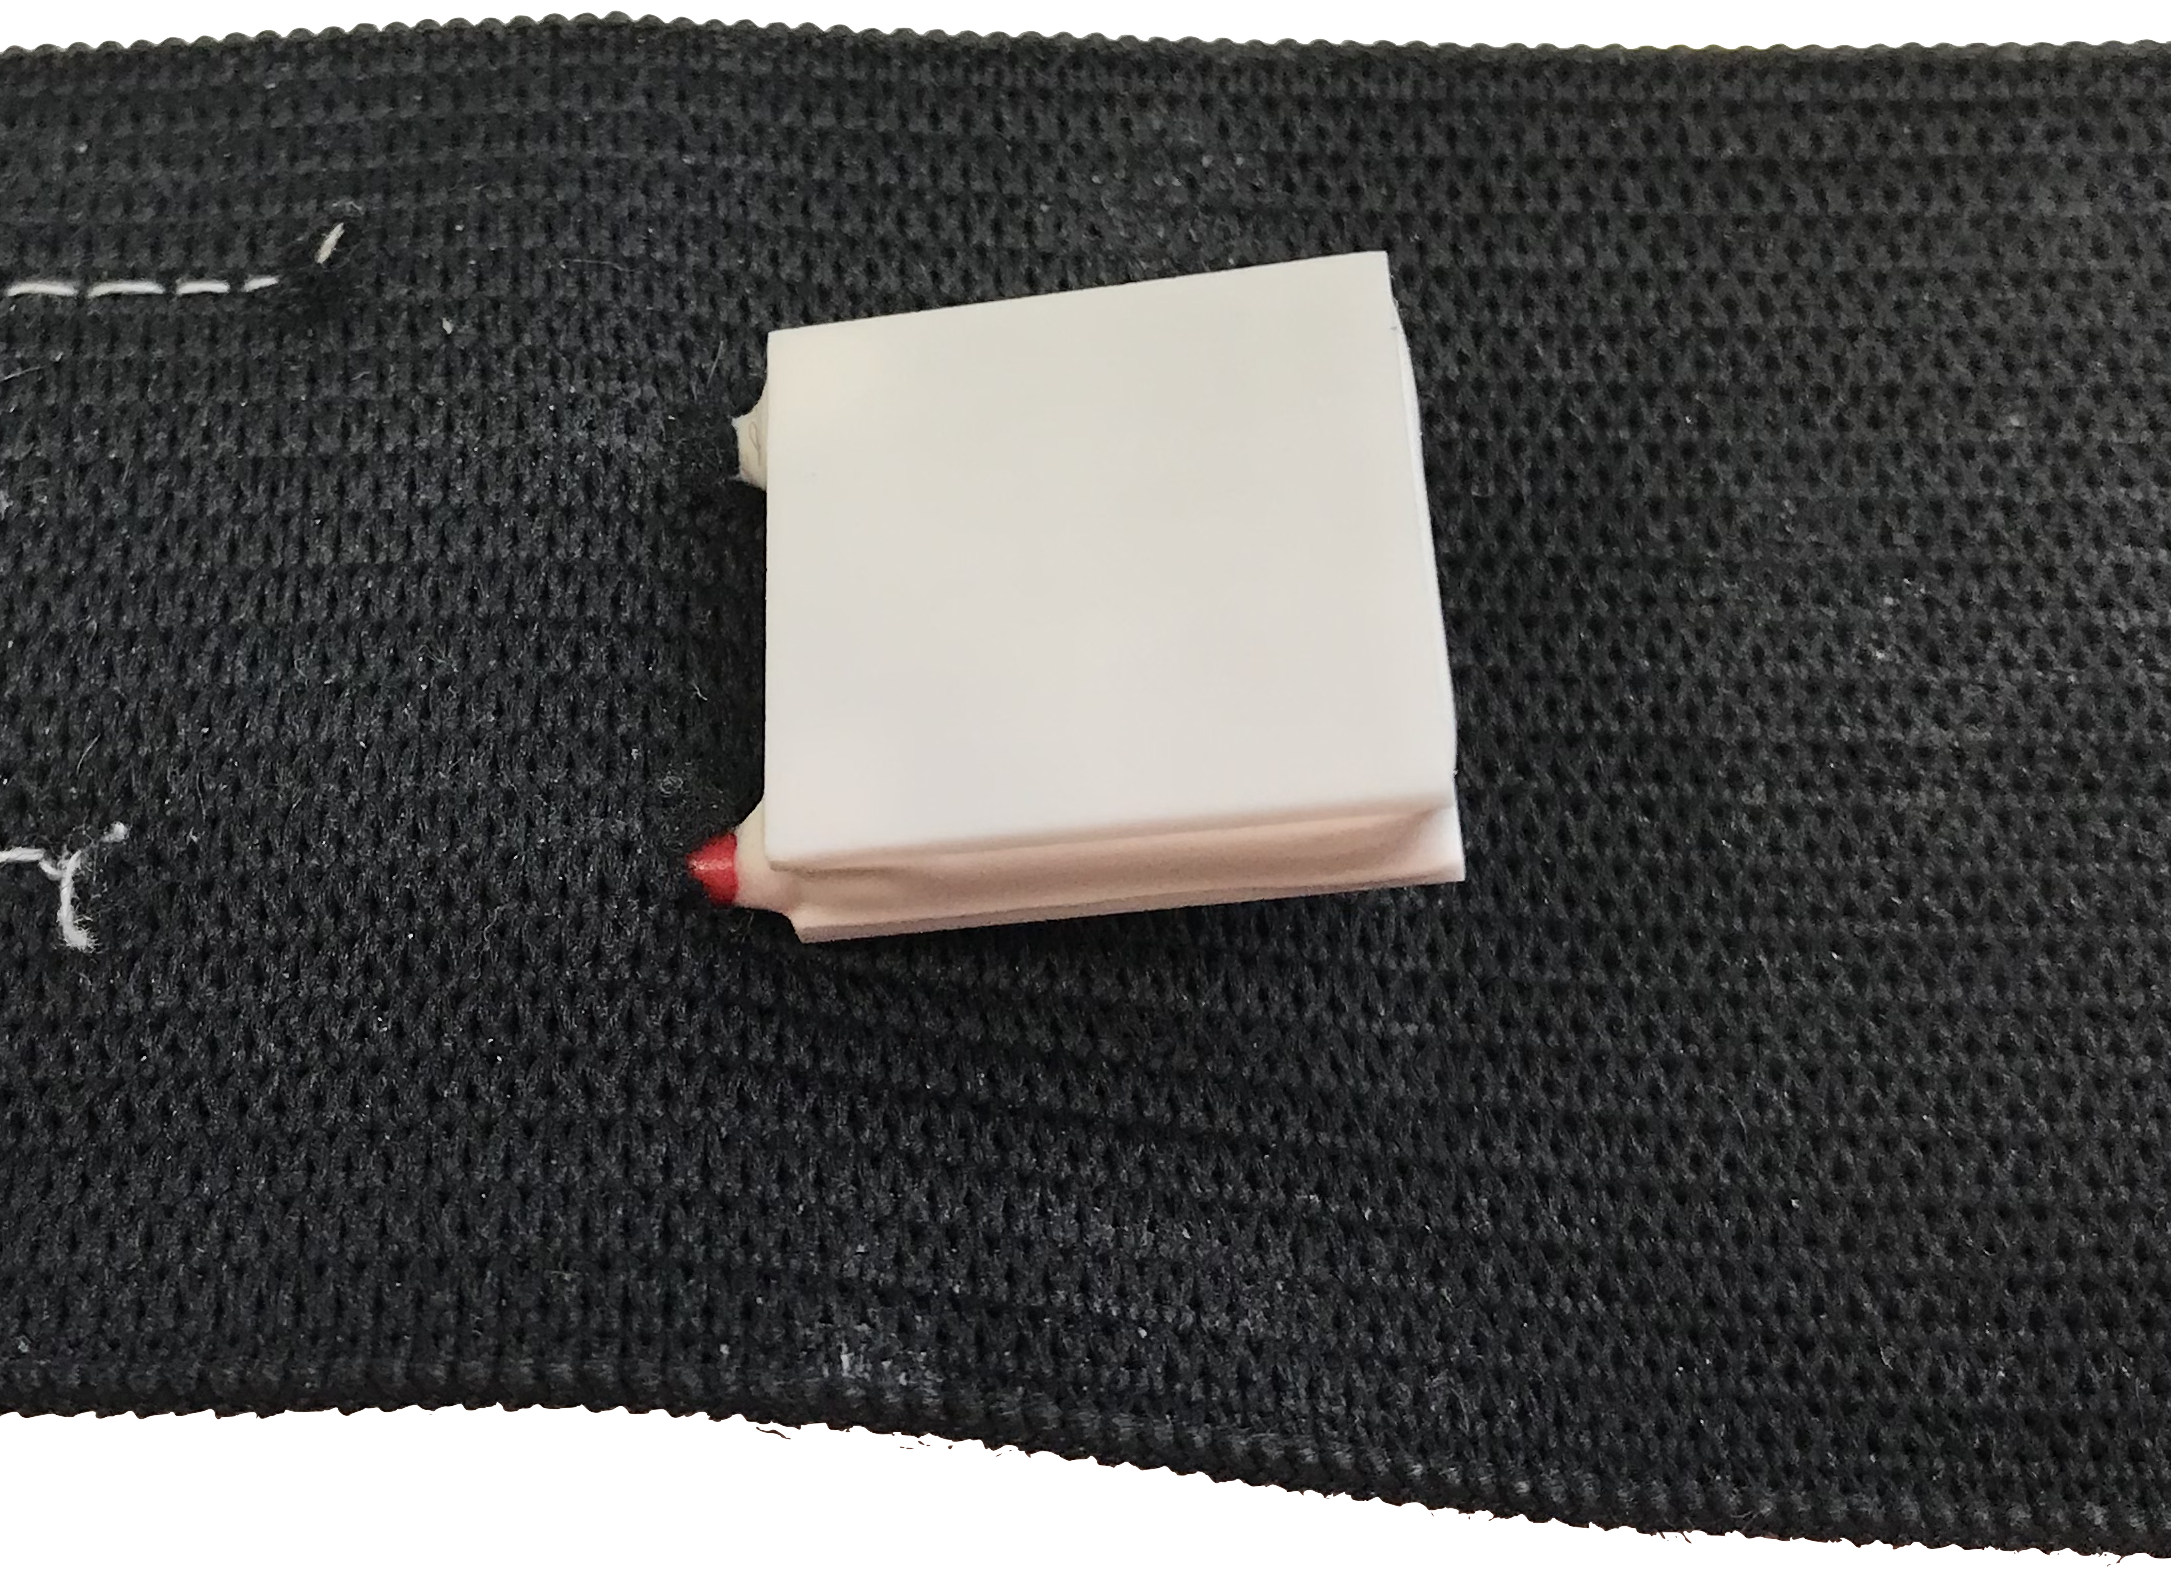
\includegraphics[width= \textwidth]{images/peltier.png}
	\caption{Peltier element mounted to the headband to be placed directly on the users skin.}~\label{fig:peltier}
\end{figure}

As depicted in figure~\ref{fig:headbandmotorbag} a piece of the elastic band was sewn to the headband to house the vibration motor.
Since we choose an already waterproof vibration motor the only challenge is to keep the motor in place and still provide as much tactile performance to the user as possible.
Therefore the the piece of elastic band is sewn to the headband to be at maximum stretch when the motor is in the bag.
The kinetic energy is better transferred by rigid objects.
As for the Peltier element, the motor is not perceived by the user wearing the headband while it is turned off.

\begin{figure}
	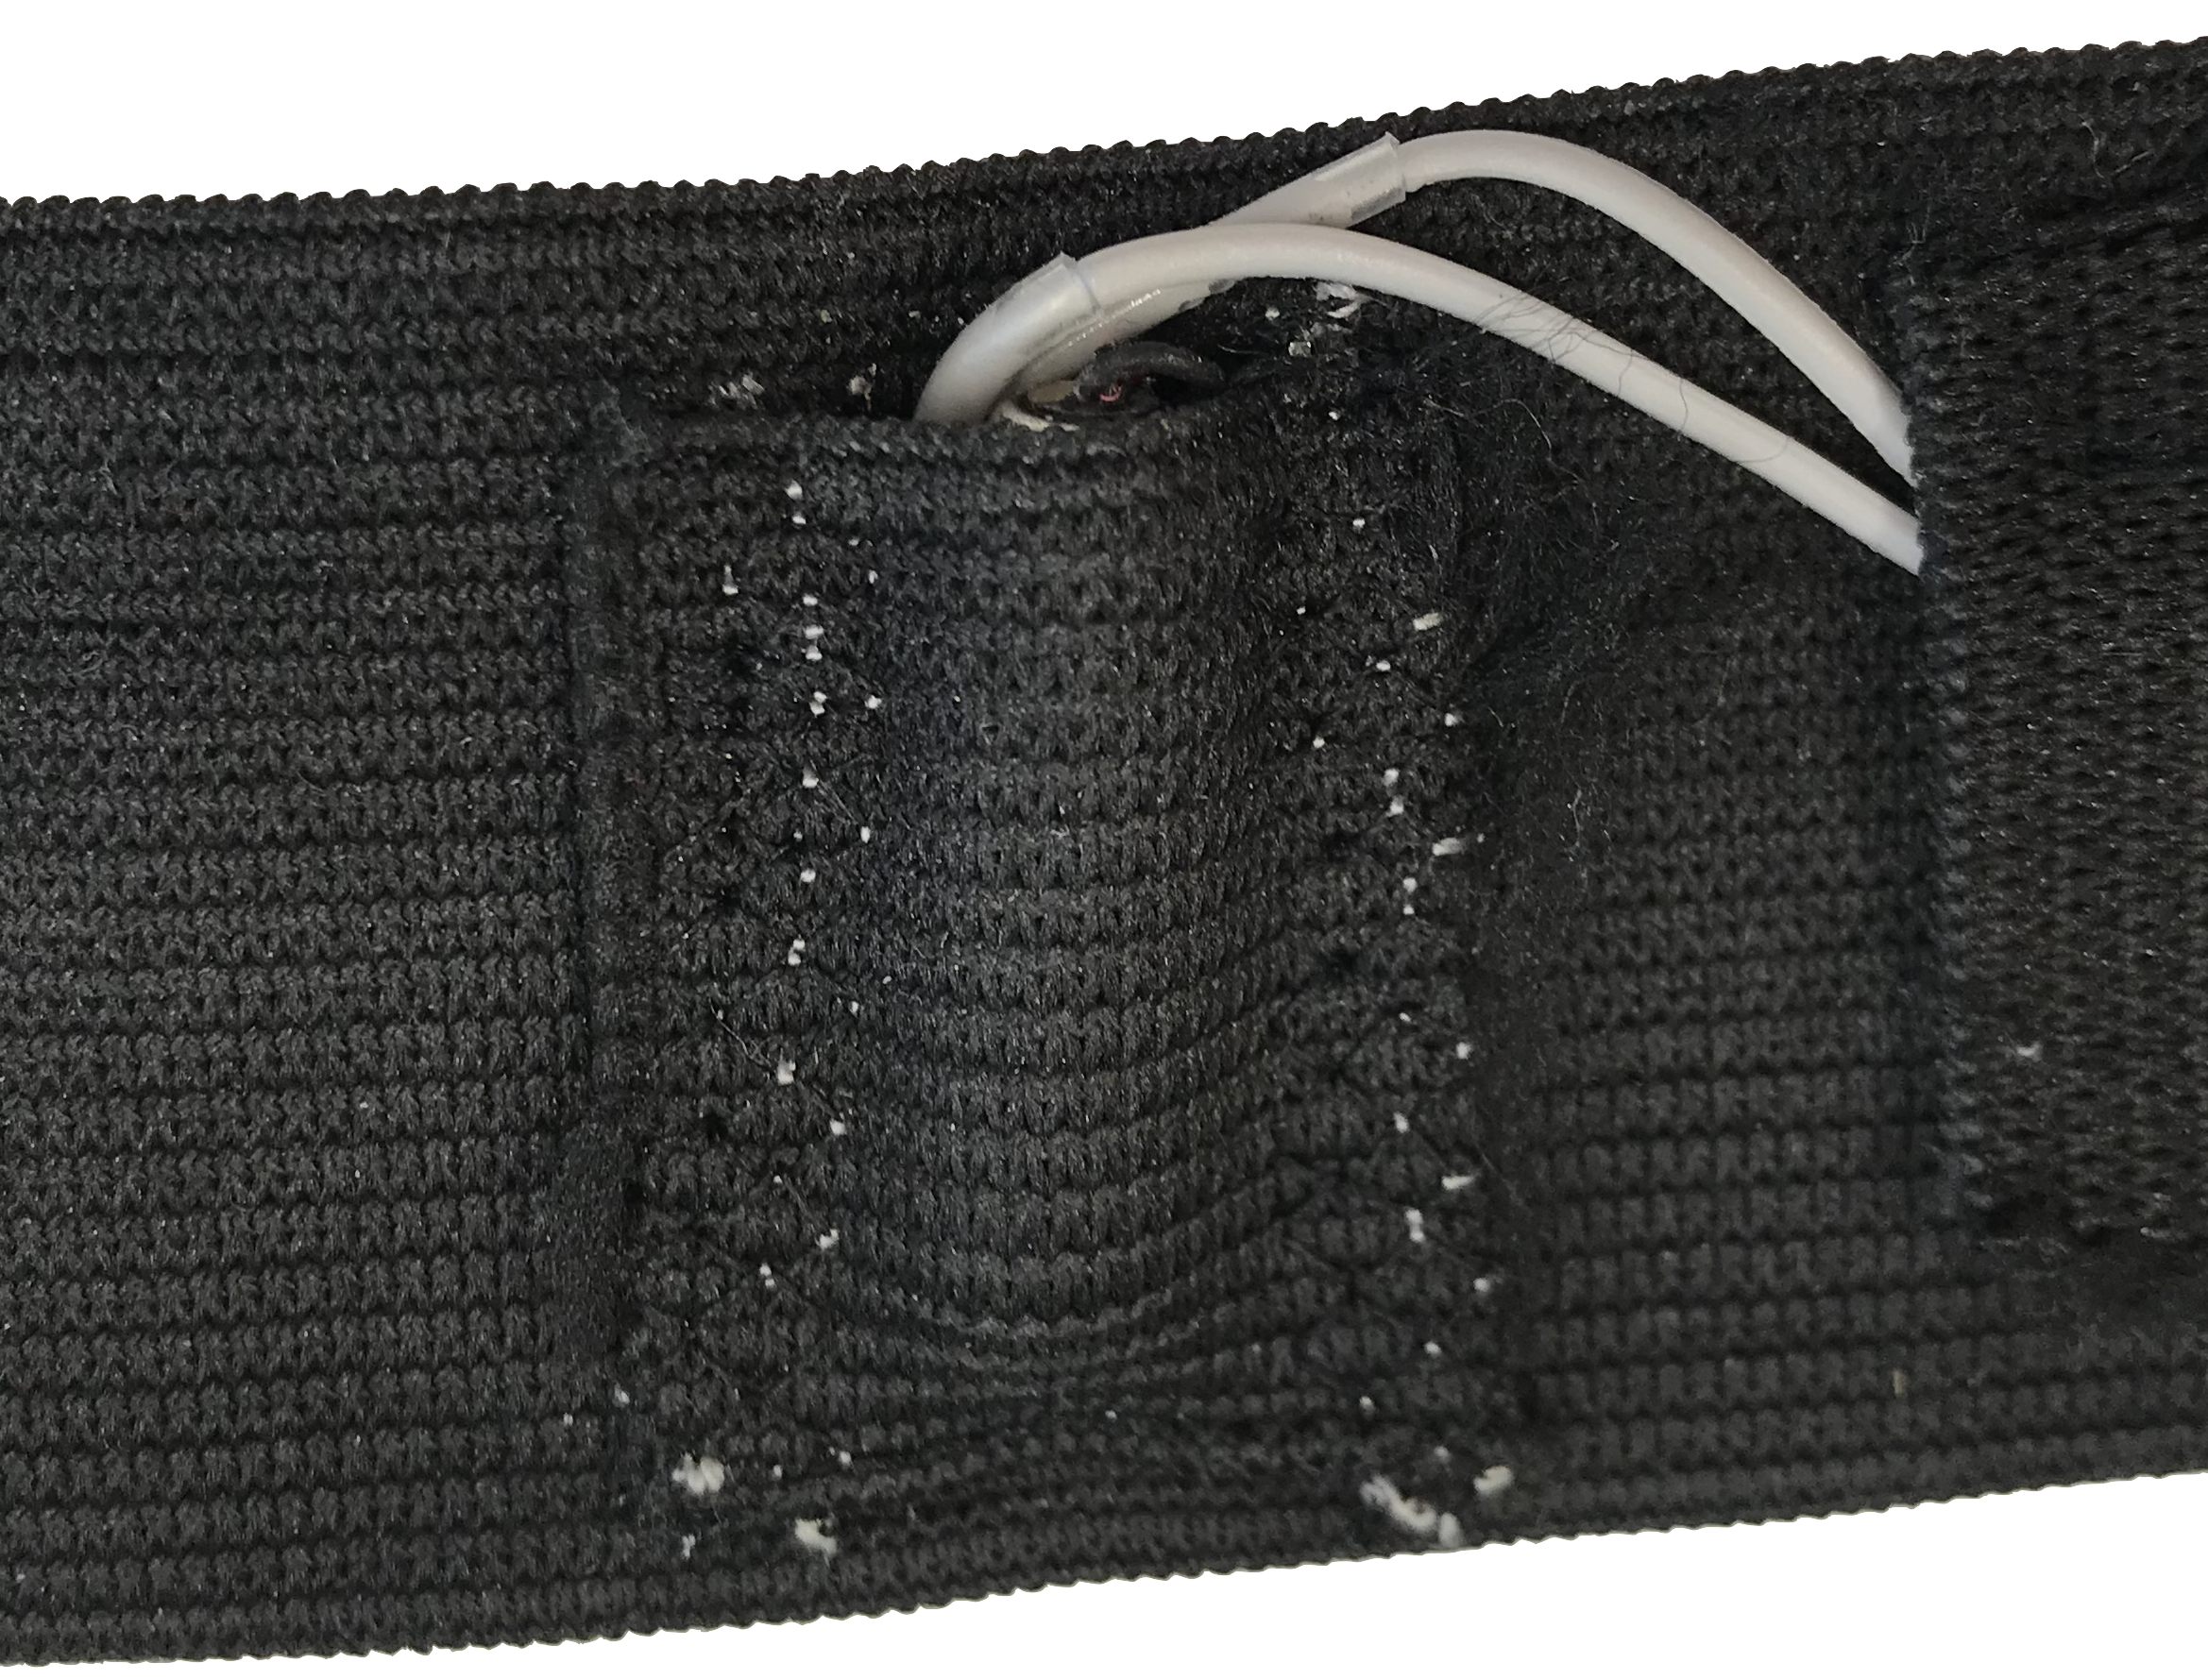
\includegraphics[width= \textwidth]{images/headbandmotorbag.png}
	\caption{Piece of the stretchband sewn to the headband as a bag for the vibration motor.}~\label{fig:headbandmotorbag}
\end{figure}

To prevent the user form tangling up in the wires we sew pieces of the elastic material to the headband as shown in figure \ref{fig:headbandpatches}.
These wireways leading to one side of the headband make wire management easier and prevent them from being damaged.

\begin{figure}
	\includegraphics[width= \textwidth]{images/headbandpatches.png}
	\caption{Pieces of the stretchband sewn to the headband as wireway for better management of the wires.}~\label{fig:headbandpatches}
\end{figure}

The user has to provide feedback if she notices one of the possible kinds of feedback we present to her.
Figure~\ref{fig:button} shows the button we use for that purpose.
We pick a large button used in arcade cabinets and a 3D printed case. 
The button features vertical lift to prevent accidental pressing by the user. 
Furthermore, the supervisor can hear a clearly recognizable click sound when the button was pressed which helps monitoring the functionality of hardware and software.
A consequence of this button design is that the user has to press it outside the water.
This is no issue since the user will stay at the pool edge anyway.

\begin{figure}
	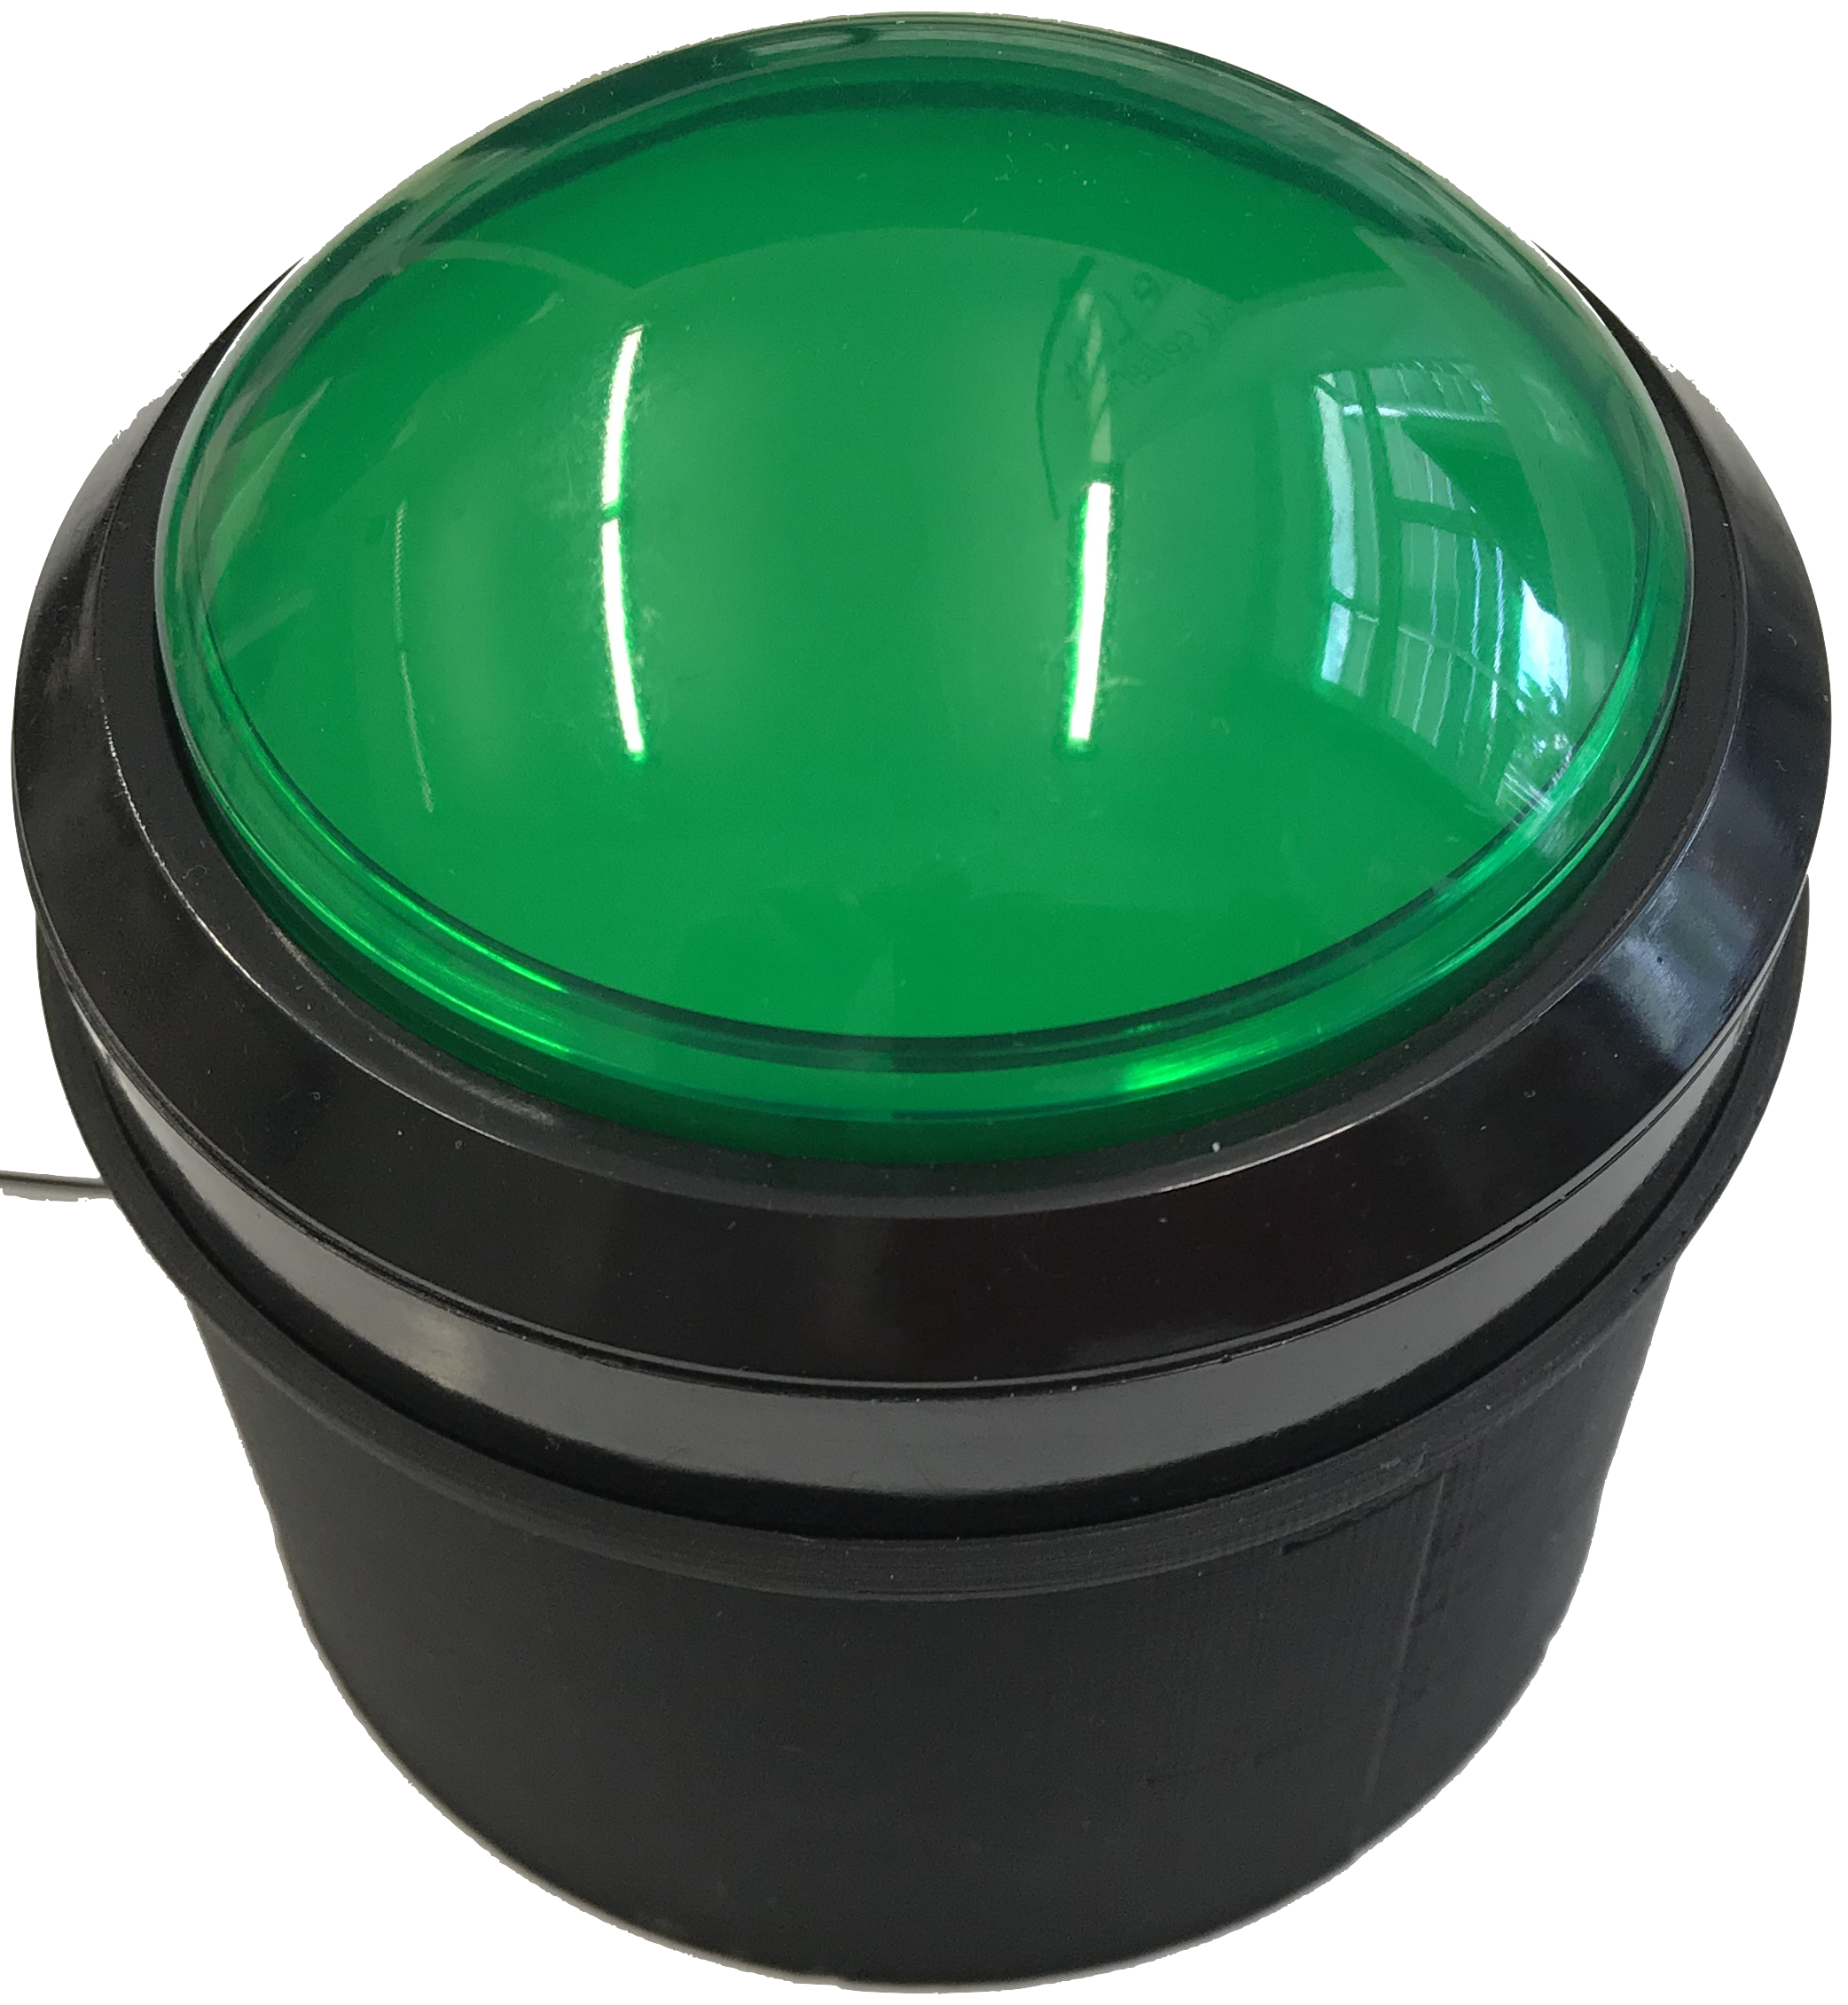
\includegraphics[width= \textwidth]{images/button.png}
	\caption{The botton and the 3D printed case. To be pressed by the user when he recognizes feedback.}~\label{fig:button}
\end{figure}
\todo{length of ribbon cable} 
The wires of the LED, vibration motor, Peltier element, and botton are joined with a ribbon cable depicted in figure~\ref{fig:wires}.
As for all connections and soldering joints, they are made waterproof with glue and shrinking tube.
The ribbon cable leads to the breadboard shown in figure~\ref{fig:breadboard}.
The breadboard houses an Arduino Uno, the cables leading form the pins to the ribbon cable, a relay, and a battery case.
The relay is connected to the Arduino Uno  which controls when it connects the two AA batteries with the Peltier circuit.


\begin{figure}
	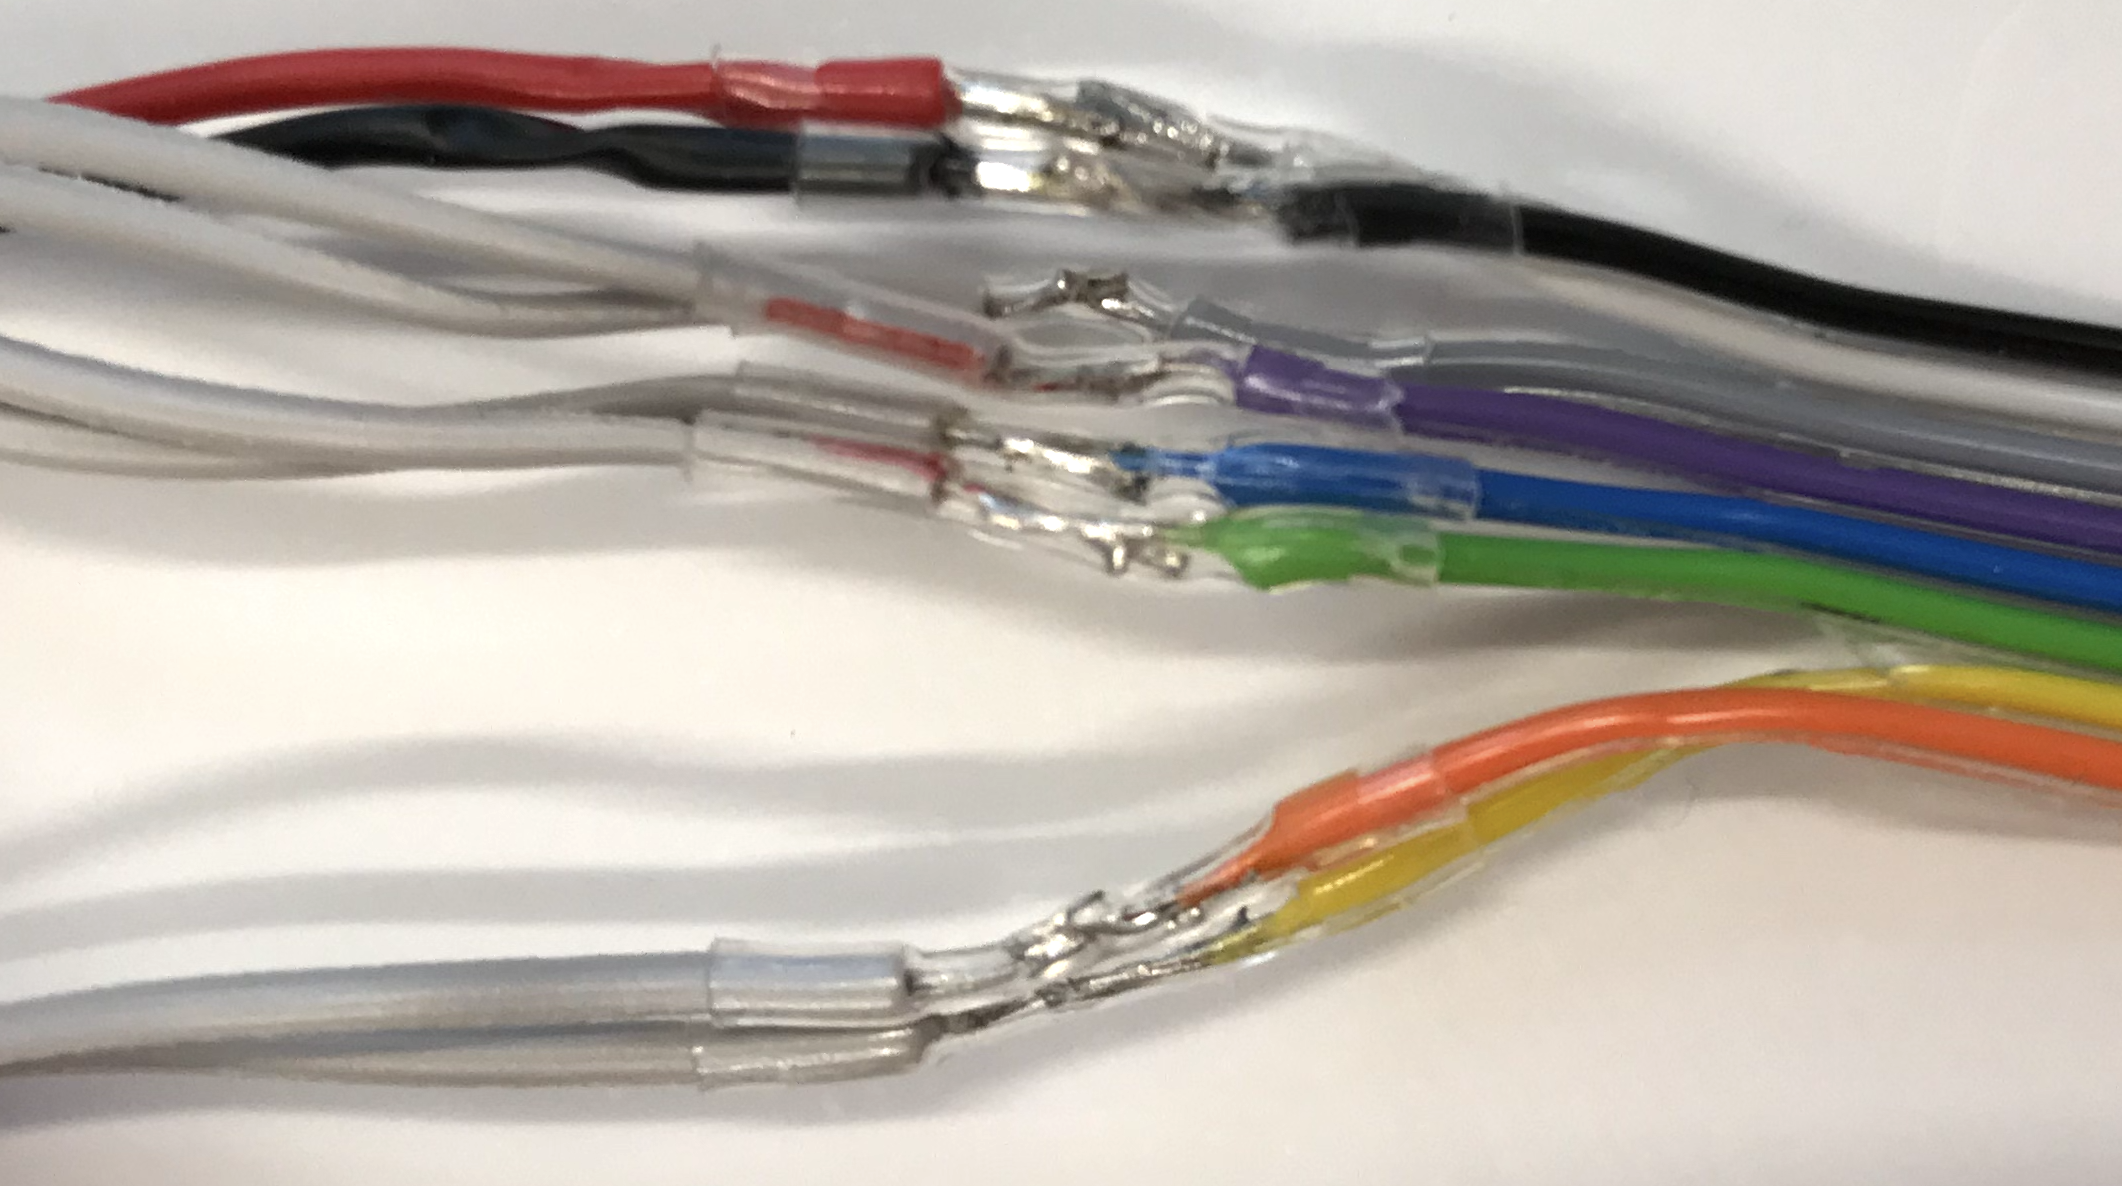
\includegraphics[width= \textwidth]{images/wires.png}
	\caption{Waterproof join of wires from each actuator to the ribbon cable.}~\label{fig:wires}
\end{figure}

\begin{figure}
	\includegraphics[width= \textwidth]{images/breadboard.png}
	\caption{The Arduino controlling the relay and other components of the prototype via the ribbon cable. The batteries power the Peltier element when the relay is set correspondingly.}~\label{fig:breadboard}
\end{figure}


Figure~\ref{fig:studysetupcut} shows all prototype parts worn by the user.
 
\begin{figure}
	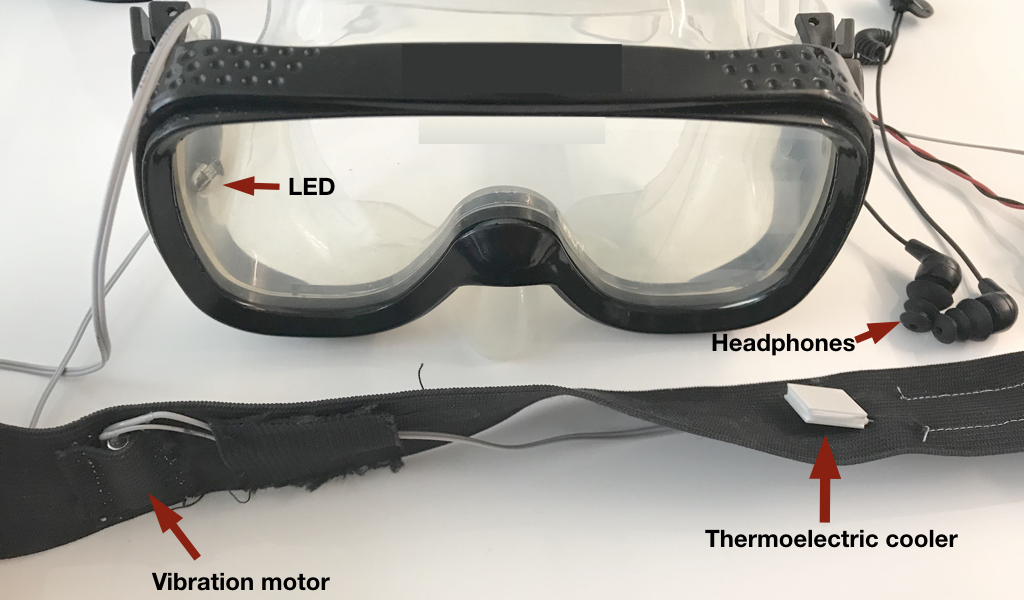
\includegraphics[width= \textwidth]{images/studysetupcut.png}
	\caption{Headband, diving goggles, and waterproof headphones with the integrated LED, Vibration motor, and Thermoelectric cooling module.}~\label{fig:studysetupcut}
\end{figure}


\subsection{Safety}

Since we operate electronics in an underwater test environment, safety concerns arise.
In fact, the voltage and current are below critical values.
Besides, all  wired connections are waterproof and tested for three days in a box filled with water.
The breadboard is always placed in some distance and above the water surface.
During the operation of the prototype in underwater scenario the breadboard and batteries are loosely covered by a towel to protect it against splashing water.

\todo{pin header sizes}
In case the user leaves the pool edge the ribbon cable falls off the breadboard rather than pulling it down. 
We achieve this with shorter than usual pin headers connections.

\section{Software}

The  software for the prototype and the user study runs partly on the Arduino Uno micro controller and partly on a computer.
The micro controller activates the feedback elements or signals the computer to via processing to play a sound file. 
Furthermore it tracks the time a user needs to press the button after the feedback was activated and sends that date to computer.
Processing receives the data frames from the micro controller and creates a file to log the data for further analysis or plays the sound file and tracks that time.

\paragraph{Arduino Code}
Each stimulus (increasing LED, LED, increasing vibration, vibration, sound, peltier element) is exclusively encoded with a number from \emph{0} to \emph{5}.
Six distinct arrays were randomly generated only limited by prohibiting occurrences of the same stimuli in a row more than two times and by making sure each stimuli is active exactly 8 times.
This results in 48 stimuli per program run.
The random generation of the arrays is used to prevent participants from recognizing the order of the stimulus which might influence the results.
It has been done in a  separate program to due to an inefficient algorithm which would slow down the user study program unnecessarily.

The program iterates over the array and a \emph{switch case} statement the triggers the corresponding actions.
For each action the time is saved in milliseconds immediately before the stimulus is activated.
The program proceeds with the current action until the button is pressed and the start time is subtracted from the end time.
Results are sent in a format which specifies whether data (\emph{D}) follows, the sound file (\emph{S}) has to be played, or an interrupt (\emph{I}) via a button press was issued after the sound file was played. 
This is followed by the identification number of the action.
Thereupon follows the time (\emph{t}) in milliseconds and a \emph{x} to terminate the frame or just the \emph{x} if it is not data.
Tracking the time of the sound is done on the computer.
For example a data frame after the LED action is completed in 0.45 seconds looks like \emph{D3t450x}, a play-sound frame like \emph{S5x}, and when the button was pressed while the sound file is playing like \emph{Ix}.

After each action is completed the program waits for two seconds and additionally a random number of seconds between zero and five before the next action triggers.
This is done to further prevent the users' adoption to a rhythm which influences the measurements.
Once the 48 actions are completed \emph{Fx} is sent and the program enters an infinite loop.

\paragraph{Processing Code}
In Processing we create a Writer which creates and writes to a text file for logging the user study data.
Furthermore a sound file is loaded to be played when the corresponding signal from the micro controller arrives. 
Processing reads the incoming data from the micro controller per character and saves it in an char array. 
If \emph{x} is read, the serial port is cleared and the data handling begins. 
In case of a data transmission for the LED, vibration motor, or peltier element, the identification number of the current stimulus and the corresponding time is written to the log file. 
If S is received the sound file is played and the time is saved as on micro controller. 
After pressing the button playback of the sound file stops and the time taken is calculated and written to the logfile. 
After handling the data the buffer is cleared and the next data frame can be received. 
When the micro controller sends F to signal the end of the program the log file is saved.

\subsection{Testing}
\paragraph{Hardware testing}
To ensure the functionality of the prototype underwater and over a longer period of time testing is required. 
This is particularly important since the supervisor of the study can not tell if the prototype works properly while the participant is submerged. 
In advance of assembling the prototype we tested each component individually over several days. 
The corresponding modes for each modality were activated in intervals similar to the user study program. 
As mentioned in \ref{ownwork} we tested some vibration motors which are not suited for our needs. 
Repeated tests have shown that the small and cheaper vibration motors break after running them even outside the water. 
However higher quality vibration motors in the same small order of magnitude seem promising. 
Since the already waterproof vibration motors passed the test we went with those for the sake of convenience. 
All other components passed the testing without errors.

\paragraph{Measurement accuracy}
Since we measure in milliseconds and feedback is partly recognized in under one second we must ensure the measurements are correct. To ensure high accuracy we tested each modality and the communication latency itself. Communication latency is not measurable within the millisecond range. 
The sound file is cut such that it starts with a clearly audible noise level from the beginning. Measuring a single playback of the file reveals that there is a short delay of about 2 milliseconds. 
This delay can be considered redundant. 
Besides it is influenced by the hardware which reads and plays the file and the file size itself. To reduce the delay of the vibration motor to the same magnitude we let the vibration motor run with low rotation which is not noticeable. The increasing motor action starts precisely at an intensity which is barely noticeable outside the water. Activating the LED has no measurable delay in the millisecond range.























